\documentclass[french,12pt]{article}
\usepackage{babel}
\usepackage{a4}
\usepackage{amsmath}
\usepackage{graphicx}

\begin{document}
\sloppy

\begin{titlepage}
\begin{center}

%\setlength{\unitlength}{1in}
%\begin{picture}(0,0)
%   \put(-4.3,-10){\includegraphics{fond4.eps}}
%\end{picture}

.
\vspace{5.3cm}

\Huge \bf {POULE}

\vspace{1cm}

\LARGE
Modelisation
\mdseries

\vspace{2cm}

\large
\mdseries
\begin{tabular}{l r}
Nicolas \textsc{Metais} & Jean-Daniel \textsc{Michaud} \\
Jonathan \textsc{Mimouni} & Francois \textsc{Morlot}
\end{tabular}


\vspace{2cm}
Le \today

\end{center}
\end{titlepage}

\strut\thispagestyle{empty}
\vfill
\pagebreak
\setcounter{page}{1}
\pagebreak

Nous  presentons  ici  les  modelisations de  differentes  parties  du
projet.  La  modelisation algebrique, des  ensembles, de l'AST  et de
l'environement. Nous avons toujours considere deux points de vue, deux
visions de la modelisation. Une modelisation structurelle, plus proche
des mathematiques  et permettant a \emph{Poule}  d'etre rigoureux dans
sa   construction.   Et   une   vision  applicative,   permettant   la
representation informatique de nos donnees.

La  modelisation algebrique  a  ete inspiree  par  la modelisation  de
FOC. Sont argumentation aussi. La  volonte de separer les especes, les
collections  et  les elements  donne  a  la  modelisation une  clarete
mathematique. L'utilisation  des classes nous  permet l'utilisation de
l'heritage  et de  tous ces  bienfaits (methodes  virtuelles, liaisons
tardives ...),  et le  trait modulaire nous  a paru evident  dans la
definition d'elements de collection.

\vspace{1.5cm}

\begin{center}
\begin{figure}[!h]
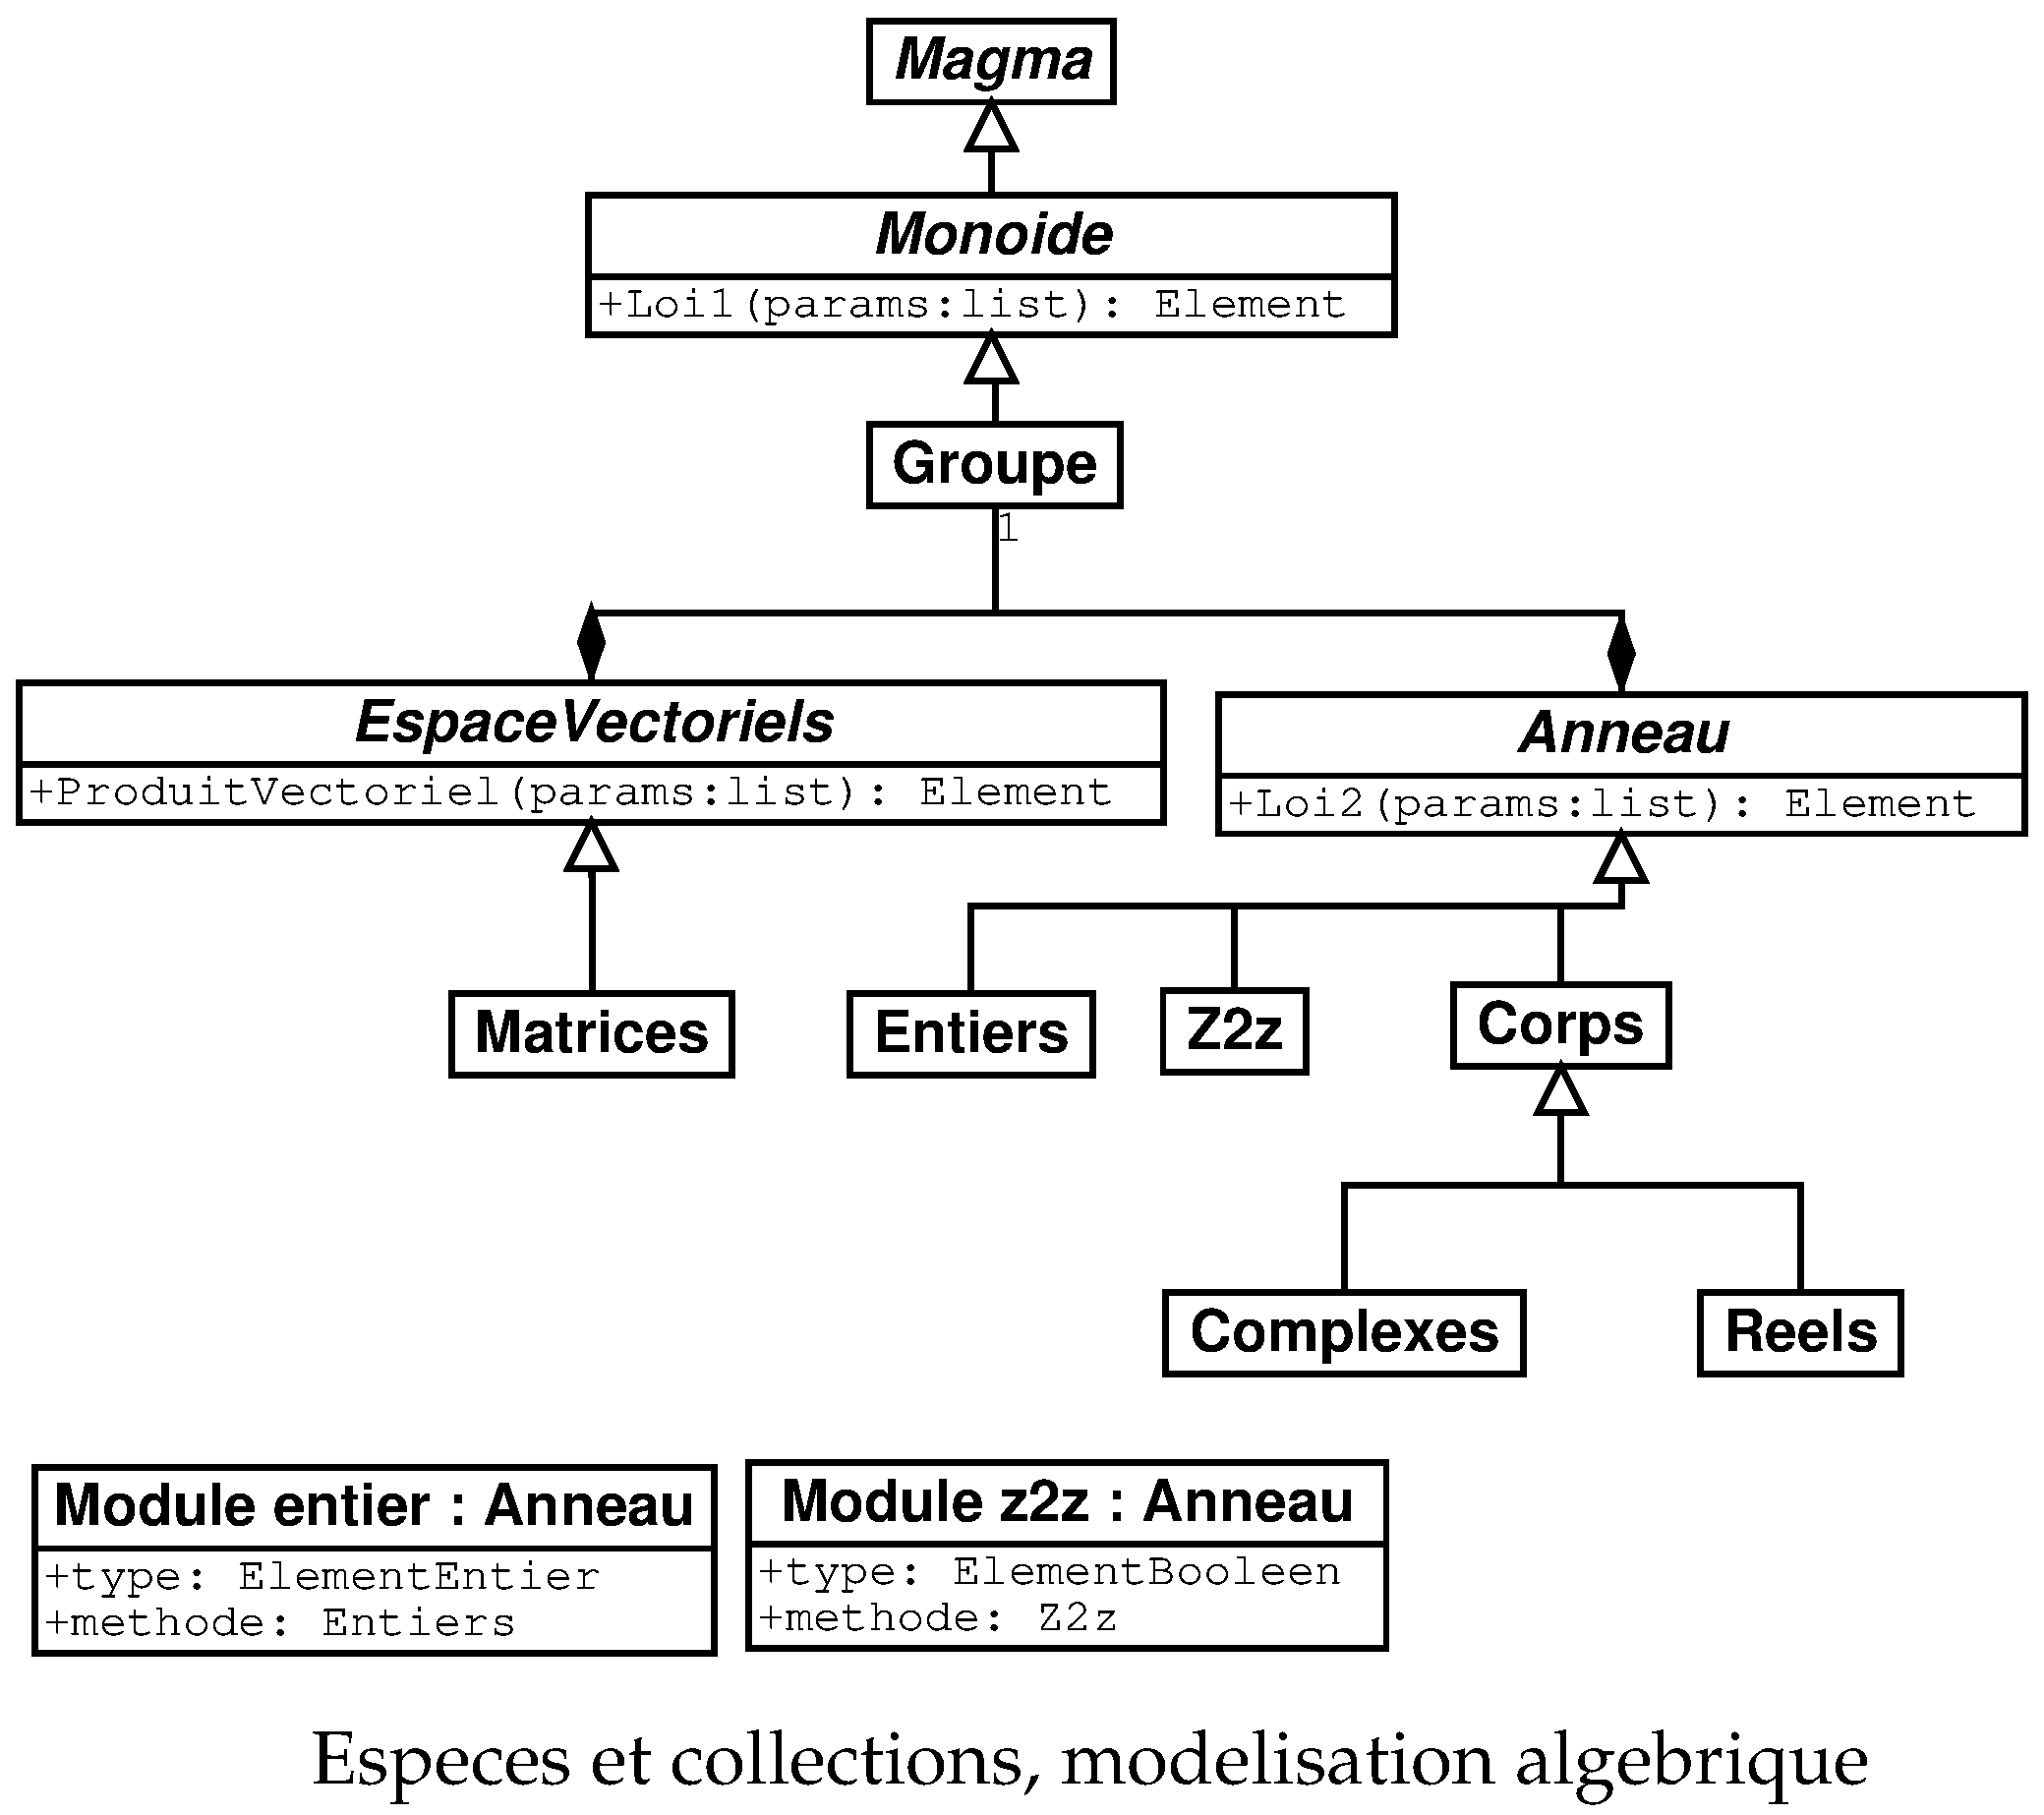
\includegraphics[width=14.5cm]{ModAlg.eps}
\end{figure}
\end{center}


La modelisation  des ensembles presentee  nous permet de  maintenir la
correspondance de  structure avec les mathematiques.  Elle nous permet
aussi  de   definir  des  proprietes  d'ensemble  et   de  laisser  la
possibilite d'en definir d'autres.

\vspace{1.5cm}

\begin{center}
\begin{figure}[!h]
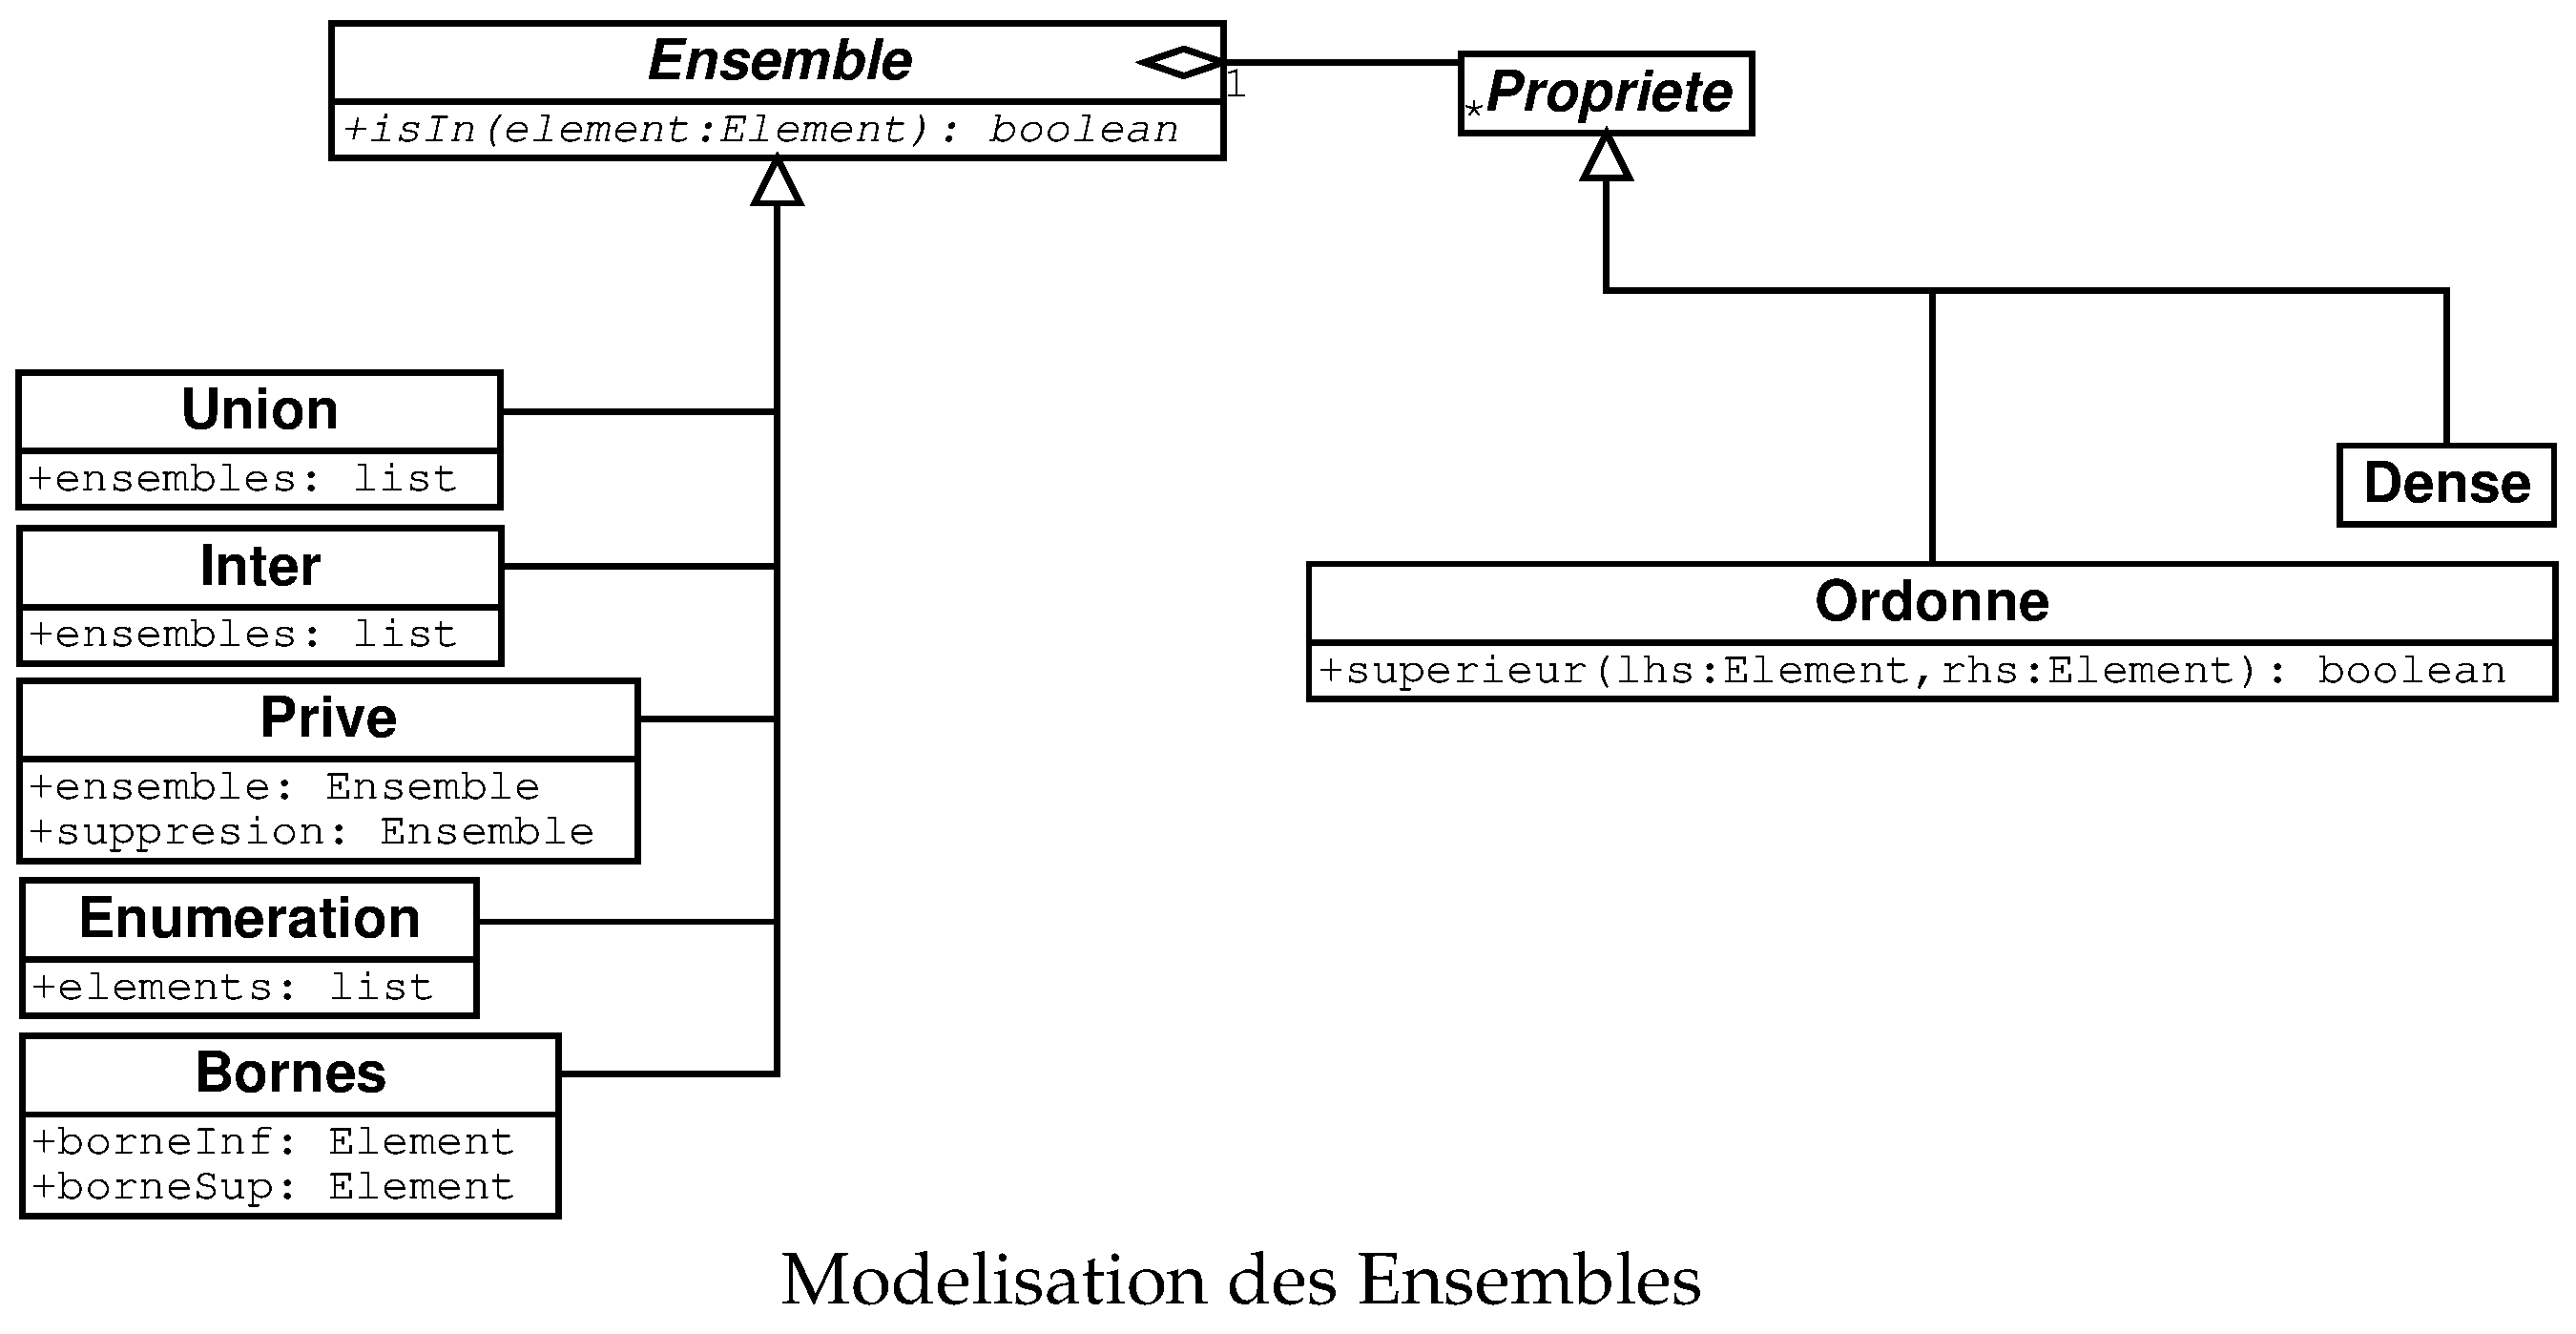
\includegraphics[width=14.5cm]{ModEns.eps}
\end{figure}
\end{center}

\pagebreak

L'AST,  directement  en relation  avec  notre  grammaire, definira  la
representation de nos donnees en memoire, la manipulation s'effectuant
sur  celui-ci, mais les  regles et  la structure  de ces  regles etant
basees sur la modelisation de l'algebre et des ensembles.

Nous definissons dans  notre AST les constantes et  les variables, les
fonctions, les operateurs et  quelques fonctions que nous qualifierons
de formelles telles que la  derivee, la primitive et l'integrale.  Les
fonctions  ne possedent  que leur  nom et  leurs parametres,  leur nom
permettant de  les extraire de  l'environement, que nous  verrons plus
tard.  Pourquoi avons  nous choisi de placer la  derivee, la primitive
et  l'integrale  dans  l'AST  ?  Car  se ne  sont  pas  des  fonctions
numeriques,  ce  sont  des  fonctions ``formelles''  agissant  sur  la
structure meme de la formule.

\vspace{1.5cm}

\begin{center}
\begin{figure}[!h]
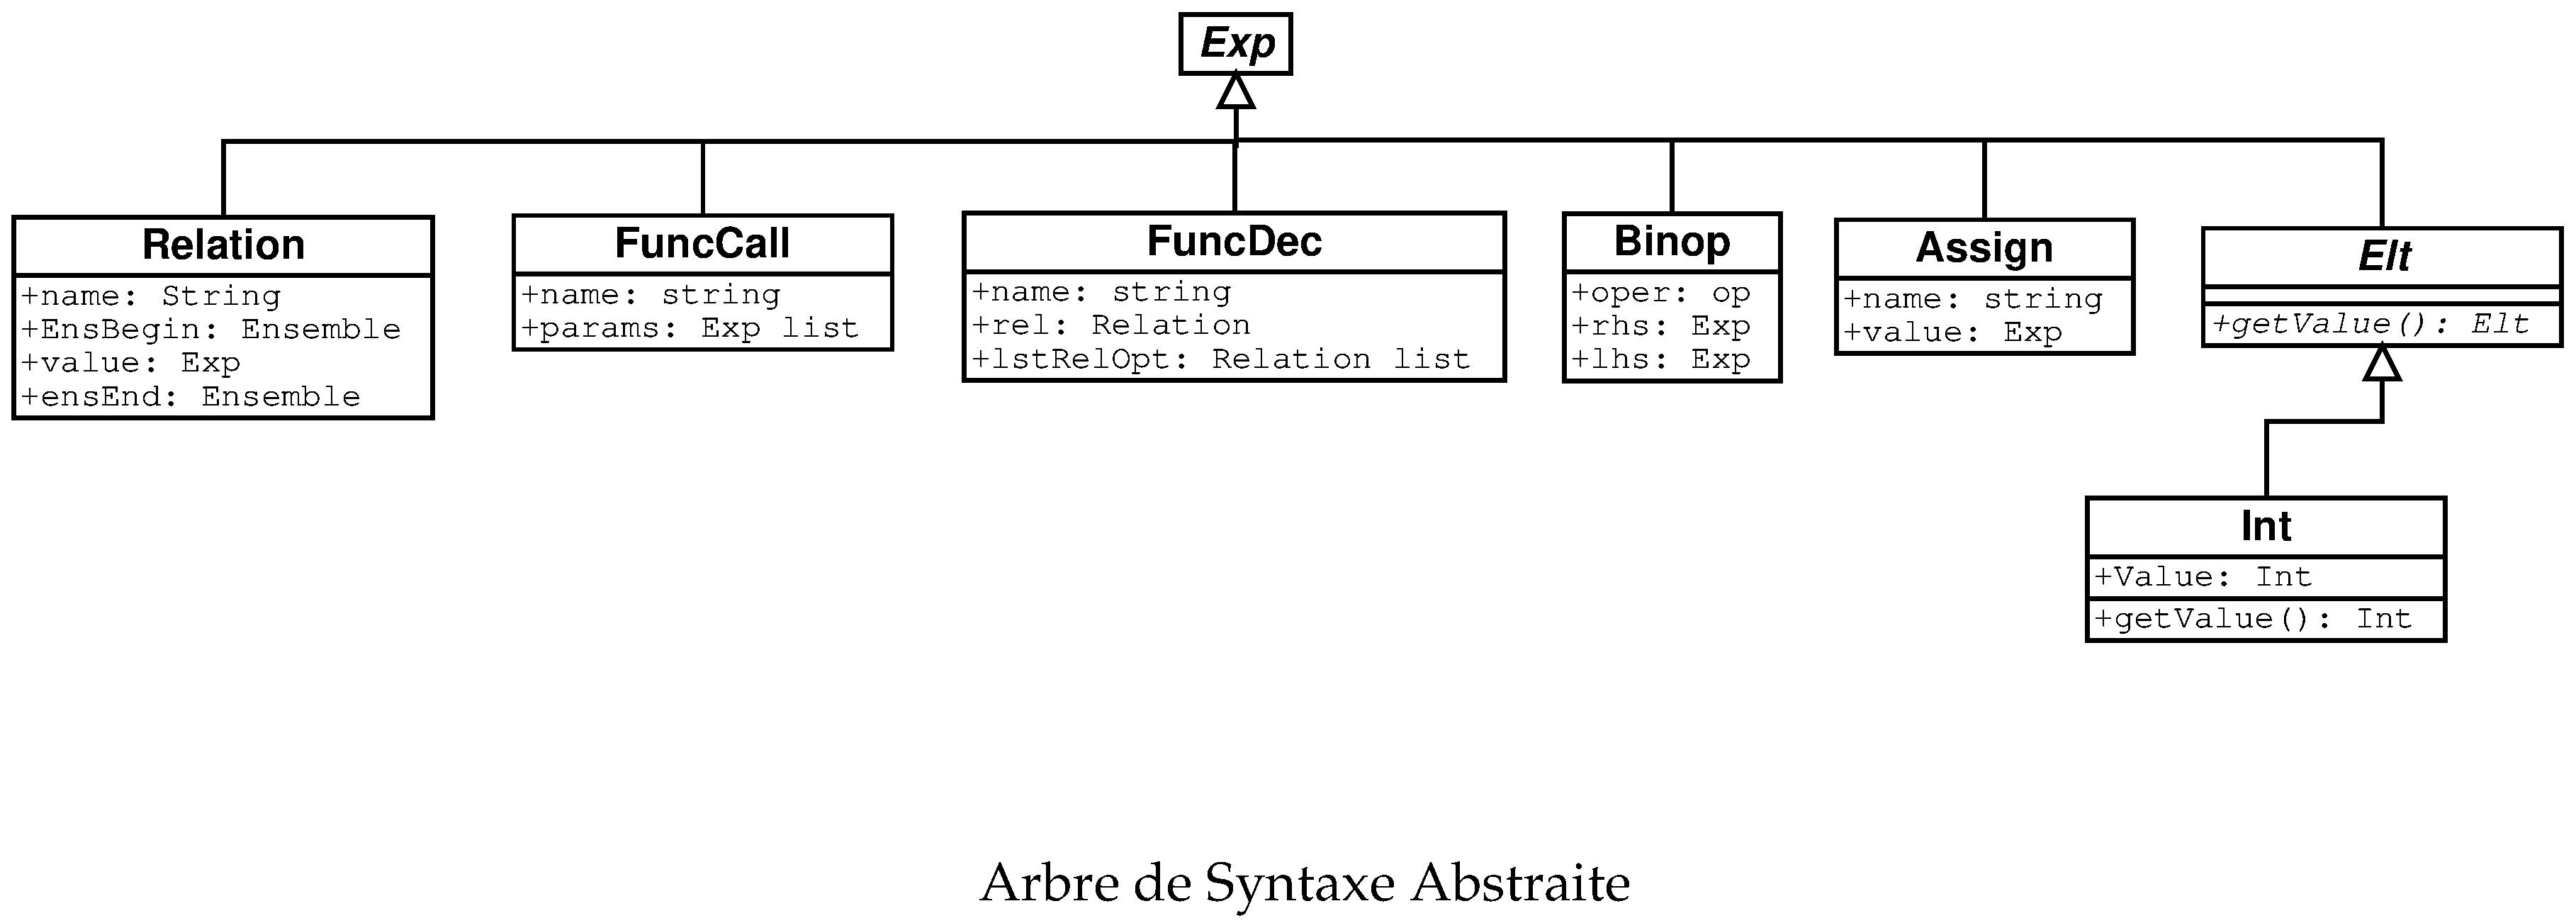
\includegraphics[width=14.5cm]{ModAST.eps}
\end{figure}
\end{center}

\pagebreak

Il nous reste a definir une modelisation pour les Entite, c'est a dire
la representation des  polynomes en vue de leur  manipulation. Et enfin
la  classe, Element.  Classe qui  n'a, pour  l'instant, pas  un avenir
certain.

\vspace{1.5cm}

\begin{center}
\begin{figure}[!h]
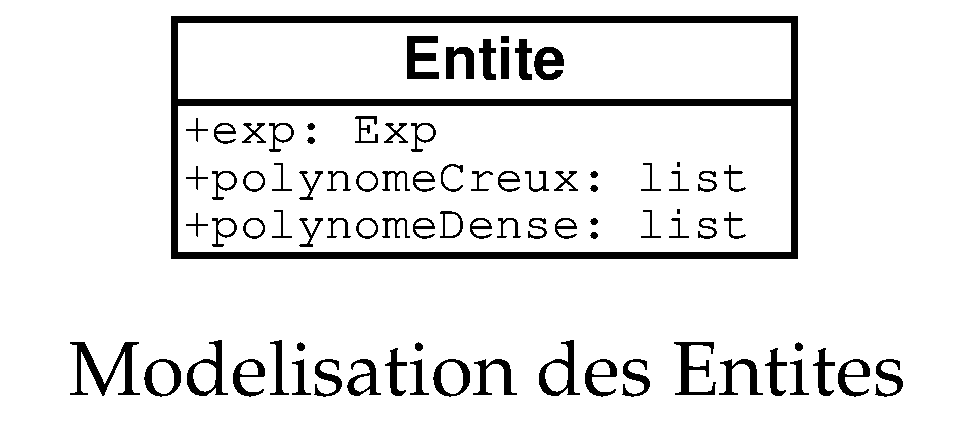
\includegraphics[width=10cm]{ModEntite.eps}
\end{figure}
\end{center}

\vspace{0.5cm}

\begin{center}
\begin{figure}[!h]
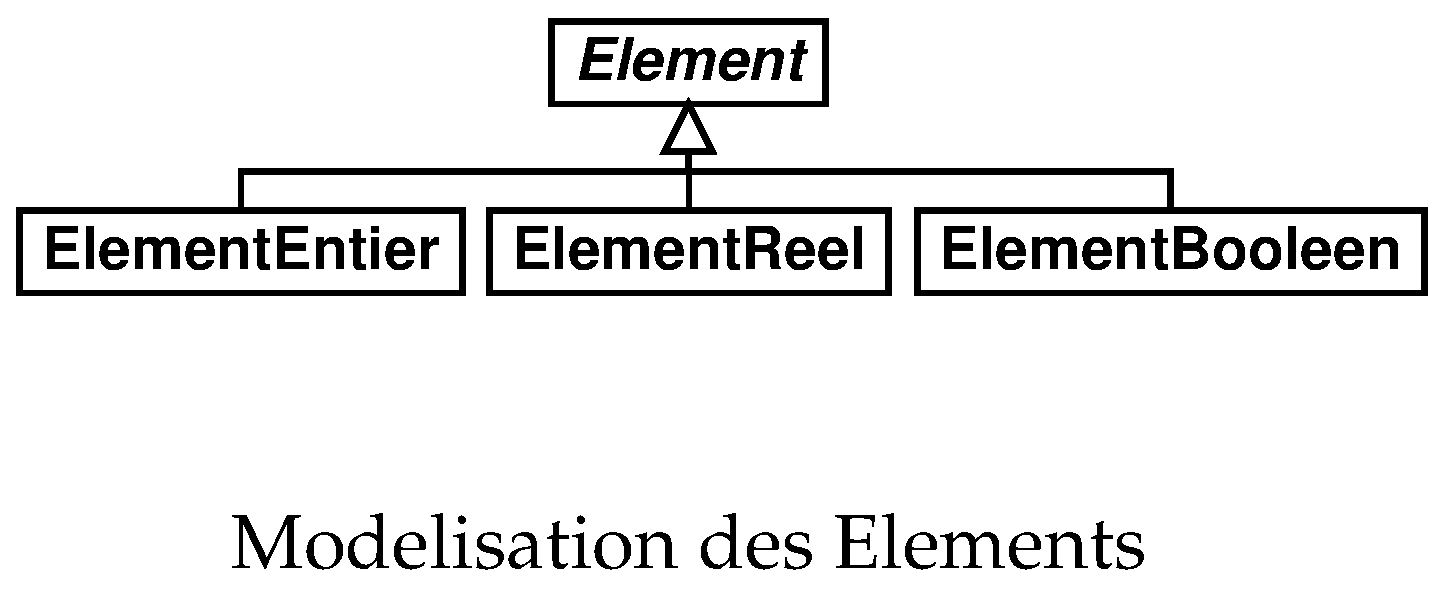
\includegraphics[width=10cm]{ModElt.eps}
\end{figure}
\end{center}

\pagebreak

Voici la grammaire:

\begin{verbatim}
digit	::=	[0-9]
entier 	::=	digit {digit}
flottant ::=	digit* '.' digit+
id	::=	[A-Za-z]+

elt	::=	entier
		| flottant
		| id 

poly	::=	elt
		| id '(' {poly} ')'
		| poly '+' poly
		| poly '*' poly
		| poly '-' poly
		| poly '/' poly
		| poly '^' poly
		| (poly)
		| derivee '(' poly, id ')'
		| primitive '(' poly, id ')'
		| integrale '(' poly, id, poly, poly ')'

Ens	::=	Ens 'Union' Ens
		| Ens 'Inter' Ens
		| Ens '\' Ens
		| ']' elt, elt '['
		| '|]' elt, elt '[|'
		| '{' elt, {elt} '}'
		| {}

params	::=	id
		| poly

Fctcall	::=	id '(' {params} ')'

Fctref	::=	Fctcall
		| poly

Fctdef	::=	id ':' Ens { '*' Ens } '->' Ens { '*' Ens }
		{id} '->' Fctref			
		[derivee '(' id ',' id ')' '->' Fctref [ 'sur' Ens ]]
		[integrale '(' id ',' id ')' '->' Fctref [ 'sur' Ens ]]

\end{verbatim}

\end{document}
